\documentclass{article}[twocolumn]
\usepackage[pdftex]{graphicx}
\usepackage[utf8]{inputenc}
\usepackage[brazil]{babel}
\usepackage{subfigure}
\usepackage{mathtools}
\usepackage{amsmath}
\usepackage{amssymb}
\usepackage{float}
\usepackage{tikz}

\title{Lab 2 - \textit{Balanced Trees}}
\author{Kenji Yamane}

\begin{document}
	\maketitle
	\section{Descri\c{c}\~ao da estrutura utilizada}
	Escolheu-se uma \'arvore rubro-negra, como sugerido no roteiro. Utilizei como refer\^encia
	somente a aula do Cap\'itulo 4, dada pelo professor Alonso, de teoria de CES-12. Ele explica
	o algoritmo para se balancear as \'arvores rubro-negras, sobre como inserir n\'os, assim
	sobre como balancear a \'arvore ap\'os a inser\c{c}\~ao, podendo realizar somente algumas
	trocas de cores ou rota\c{c}\~oes simples ou duplas dependendo de cada caso.

	Quanto \`a estrutura de classes, utilizou-se somente duas classes, uma chamada \texttt{Node},
	e uma chamada \texttt{RedBlackTree}, a qual possui uma \texttt{Node} chamada ra\'iz. A
	\texttt{Node} cont\'em mais defini\c{c}\~oes e fun\c{c}\~oes auxiliares de um n\'o de uma
	\'arvore, enquanto a \texttt{RedBlackTree} possui os algoritmos mais alto n\'ivel que
	mexem com a estrutura da \'arvore e como os n\'os est\~ao ligados.

	Utilizou-se o padr\~ao de n\'o que possui somente dois ponteiros, um que aponta para o filho
	esquerdo, e um que aponta para o filho direito. Nos algoritmos de balanceamento das \'arvores
	rubro-negras, precisa-se do pai e do av\^o. Desta forma, utilizou-se um \texttt{deque} que
	guarda todo o hist\'orico de n\'os que foram percorridos durante uma inser\c{c}\~ao. O
	\texttt{deque} n\~ao \'e limpado ap\'os cada inser\c{c}\~ao, pois isso dobraria a constante
	multiplicadora do log na complexidade. Ao inv\'es disso, suas posi\c{c}\~oes s\~ao preservadas,
	aumentando seu tamanho somente se necess\'ario, e nunca diminuindo seu tamanho.

	Al\'em da classe \texttt{Node} e da \texttt{RedBlackTree}, tem-se tamb\'em uma
	\texttt{enum class}, como recomendado no roteiro, a qual cont\'em dois atributos,
	\texttt{RED}, e \texttt{BLUE}, dispon\'ivel para ser designada para cada um dos n\'os.

	\section{Compara\c{c}\~ao com a estrutura nativa do STL}
	O teste \textit{OakByNorm} registra o tempo que cada estrutura utilizou para realizar
	ou um processo de busca ou um de inser\c{c}\~ao. Com esta informa\c{c}\~ao, tamb\'em p\^ode-se
	realizar uma regress\~ao linear com \texttt{scipy} em \textit{Python}, baseado no seguinte
	modelo:
	\begin{equation}
		y = m \log{x} + n
		\nonumber
	\end{equation}
	A regress\~ao foi feita para ambos a estrutura nativa do STL assim como para a estrutura
	implementada. O resultado est\'a na figura \ref{fig:comp_stl}.
	\begin{figure}[H]
		\centering
		\subfigure{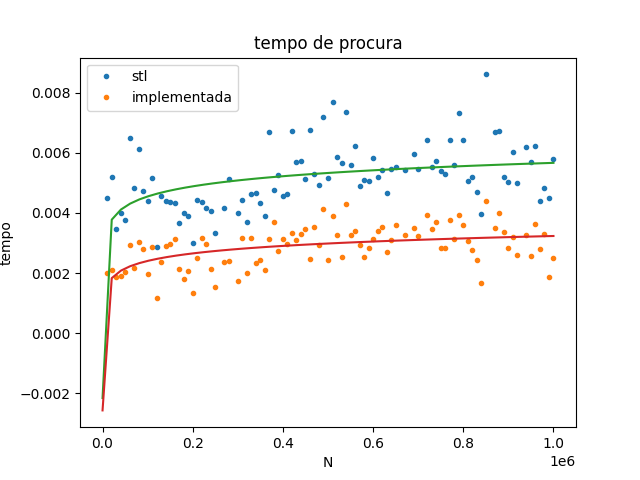
\includegraphics[width=6cm]{search_time.png}}
		\subfigure{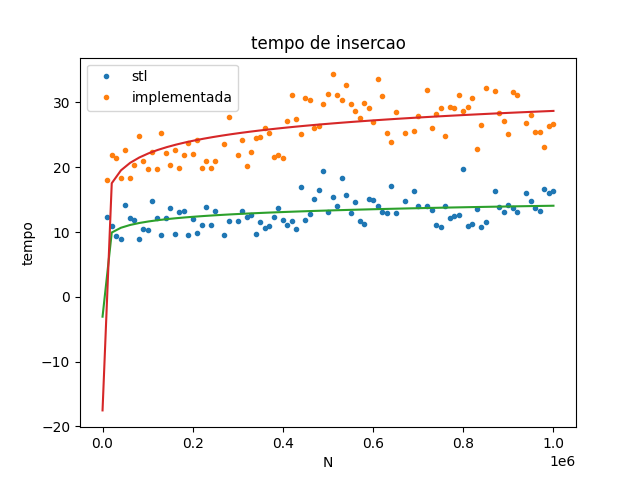
\includegraphics[width=6cm]{insertion_time.png}}
		\caption{Compara\c{c}\~ao de desempenho da estrutura criada com a nativa da STL.}
		\label{fig:comp_stl}
	\end{figure}
	Os resultados para os \texttt{r-values} de cada curva gira em torno do valor de 0,6. N\~ao \'e
	um valor t\~ao bom. Por\'em, isso foi parecido para a estrutura implementada assim
	como para a da STL, e esse menor valor pode ter sido advindo da estocasticidade gerada
	pelo teste. Visualmente e desconsiderando a estocasticidade, confirma-se que as duas curvas
	s\~ao bem condizentes com o modelo logar\'itmico. Testou-se tamb\'em com um modelo linear, e
	a regress\~ao determinava um coeficiente angular quase igual a 0, confirmando que o modelo linear
	julga as opera\c{c}\~oes quase constantes.

	\'E interessante notar que a estrutura implementada \'e melhor que a da STL na busca, por\'em
	pior na inser\c{c}\~ao. Isso \'e poss\'ivel, pois os dois algoritmos s\~ao distintos entre si.
	O algoritmo sugerido no roteiro para busca aparenta portanto ser bem otimizado.
\end{document}
